\section{Packet transactions}
Transactions are the strongest guarantee that a database system can provide in
that the effect of a transaction is either entirely visible or not with no
intermediate state being visible to the outside world.

We repurpose database transactions for data-plane programming by defining a
\textit{packet transaction}: a body of sequential code that executes from start
to finish on each packet and conceptually processes only one packet at a time.
For a programmer, the packet transaction represents what happens to every
packet without having to worry about other packets that are currently being
processed by the switch, how many pipeline stages it has, and how to
parallelize code. Conceptually, every packet is processed in isolation and to
completion using a sequential block of code before the next packet's processing
begins.

As an illustration of programming in \pktlanguage, we consider how a programmer
would express a data-plane load-balancing algorithm such as flowlet
switching~\cite{flowlet} using domino. Flowlet switching is a load balancing
that harnesses the natural burstiness of TCP traffic to load balance set of
packets (called flowlets) separated by a large enough interval in time, called
the flowlet threshold. This flowlet threshold is chosen to ensure that packets
from flowlets taking different paths do not arrive out of order at a TCP
receiver, thereby causing it to reorder packets and degrade throughput.

Flowlet switching is conceptually simple to write down and can be expressed
as the C code block shown in:
\begin{figure}[!h]
\begin{scriptsize}
\begin{lstlisting}
#define NUM_FLOWLETS      8000
#define FLOWLET_THRESHOLD 5

struct Packet {
  int sport;
  int dport;
  int new_hop;
  int arrival_time;
  int next_hop;
  int id0;
  int id1;
};

int last_time [NUM_FLOWLETS] = {0};
int saved_hop [NUM_FLOWLETS] = {0};

void flowlet(struct Packet pkt) {
  pkt.new_hop   = hash3(pkt.sport, pkt.dport, pkt.arrival_time);
  pkt.id1 = hash2(pkt.sport, pkt.dport) \% NUM_FLOWLETS;
  pkt.id0 = hash2(pkt.sport, pkt.dport) \% NUM_FLOWLETS;
  if (pkt.arrival_time - last_time[id1] >
      FLOWLET_THRESHOLD) {
    saved_hop[pkt.id0] = pkt.new_hop;
  }
  last_time[pkt.id1] = pkt.arrival_time;
  pkt.next_hop = saved_hop[pkt.id0];
}
\end{lstlisting}
\end{scriptsize}
\caption{Flowlet switching in \pktlanguage}
\label{fig:flowlet}
\end{figure}

\begin{figure*}[!t]
  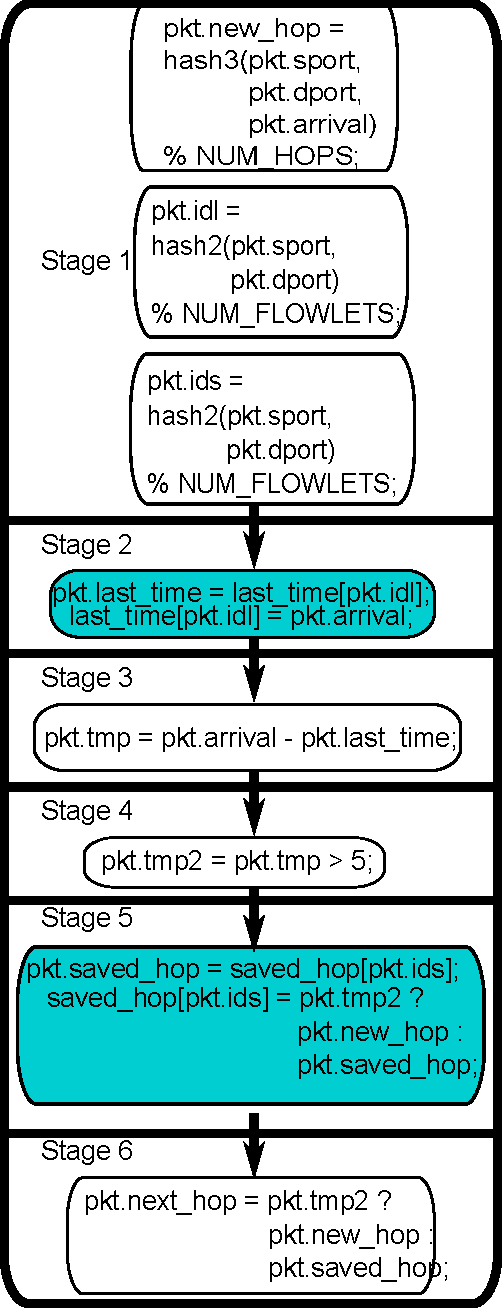
\includegraphics[width=\textwidth]{pipe.pdf}
  \caption{6-stage pipeline in \absmachine implementing flowlet switching}
  \label{fig:pipeline}
\end{figure*}

This packet transaction demonstrates the core language constructs in
\pktlanguage. All packet processing happens in the context of a packet
transaction (the function \texttt{flowlet}), a C function that takes a packet
struct as an argument. The function body of a packet transaction can reference
only two types of variables. Packet variables are represented as structure
members and persist only over the duration of a packet, e.g.
\texttt{pkt.next\_hop}). State variables are represented as global variables
and persist across packets, e.g. \texttt{last\_time}.

The function body may also call out to opaque functions such as \texttt{hash2}
and \texttt{hash3} that represent hardware primitives provided by the abstract
machine. The \pktlanguage compiler knows the function's signature and uses
these to infer dependencies, but doesn't know anything about its
implementation. Finally, the function body is written in a constrained subset
of C that excludes all iterative constructs. The function body can include if
and else-if statements, but all other control transfer (break, goto, switch,
return, and continue statements) is forbidden. Lastly, \pktlanguage forbids
pointers and dynamic memory allocation. Arrays can be used as state variables,
but in a restriced form: for a given array, all accesses to the array must use
the same address for a given packet.

These restrictions may seem severe at first glance, but are required to provide
deterministic performance guarantees. Further, we show (\S\ref{s:eval}) that
\pktlanguage can still express several data-plane algorithms  of practical
interest at a much higher level of abstraction than possible today.

When compiled to the \absmachine abstract machine (\S\ref{s:machine}), the
\pktlanguage compiler converts the code in Figure~\ref{fig:flowlet} into the
pipelined form shown in Figure~\ref{fig:pipeline}. Today, programmable switch
chips are programmed by manually specifying pipeline configurations resembling
Figure~\ref{fig:pipeline} using a language like P4 or an API such as Cavium's
XPliant SDK. Programming in \pktlanguage lets a compiler automate this process:
the user doesn't worry about hardware details such as pipeline stages and
concurrency within each stage.

Expressing code using packet transactions also allows to check for correctness
of compilation, by feeding the same test input into both the transactional code
block (Figure~\ref{fig:flowlet}) and its pipelined implementation in
\absmachine and checking that the outputs are identical for both the
transactional specification and its pipelined implementation. We describe our
test framework, \tester that uses this idea to validate the correctness of
compilation of all our test programs.

% Anirudh->Alvin: Maybe move grammar into appendix?

% Anirudh->Alvin: I think we might want to get rid of a language section and
% just describe the language as part of this example itself?
%%Additionally,
%%\pktlanguage currently only handles scalar packet variables
%%Permits arrays with the same read and write addresses.

%The global arrays \texttt{last\_time} and \texttt{saved\_hop}
%represent the last time a packet was received from a given 5-tuple and the
%saved value of the next hop for that 5-tuple.\footnote{Hash function collisions
%  can occur, leading to two flows sharing last\_time and saved\_hop values. As
%we explain later in \S\ref{s:banzai}, this is unavoidable given the constraints
%on modern switch architectures.}. The next\_hop packet field specifies the next
%hop chosen for the packet, which can either be the saved value of next hop or a
%newly computed value.
